\documentclass[journal,10pt,twocolumn]{article}
\usepackage[margin=0.5in]{geometry}
\usepackage[cmex10]{amsmath}
\usepackage{array}
\usepackage{booktabs}

% The preceding line is only needed to identify funding in the first footnote. If that is unneeded, please comment it out.
\usepackage{cite}
\usepackage{amsmath,amssymb,amsfonts}
\usepackage{graphicx}
\usepackage{textcomp}
\usepackage{xcolor}
\usepackage{graphicx}
\graphicspath{{./fig}}{}
\def\BibTeX{{\rm B\kern-.05em{\sc i\kern-.025em b}\kern-.08em
    T\kern-.1667em\lower.7ex\hbox{E}\kern-.125emX}}

\usepackage{tikz}
\usetikzlibrary{shapes.geometric}
\usetikzlibrary{shapes.geometric,angles,quotes}

\usetikzlibrary{positioning,fit,calc} % used for the efficient working of the positioning system  
\tikzset{block/.style={draw, thick, text width=3.5cm, minimum height=1.5cm, align=center},   
% the align command is used to align the block diagram at the center  
% the height command adjust the height of the block diagram  
% here block diagram refers to the whole diagram, not the single block  
% the thick command here signifies the border of all the blocks used inside the block diagram. You can change it to thin command if you want the thin edge of the blocks  
line/.style={-latex}   % the lesser the width the greater will be the diagram window  
}  

\begin{document}

\newtheorem{theorem}{Theorem}[section]
\newtheorem{problem}{Problem}
\newtheorem{proposition}{Proposition}[section]
\newtheorem{lemma}{Lemma}[section]
\newtheorem{corollary}[theorem]{Corollary}
\newtheorem{example}{Example}[section]
\newtheorem{definition}[problem]{Definition}
%\newtheorem{thm}{Theorem}[section] 
%\newtheorem{defn}[thm]{Definition}
%\newtheorem{algorithm}{Algorithm}[section]
%\newtheorem{cor}{Corollary}
\newcommand{\BEQA}{\begin{eqnarray}}
\newcommand{\EEQA}{\end{eqnarray}}
\newcommand{\define}{\stackrel{\triangle}{=}}
\newcommand*\circled[1]{\tikz[baseline=(char.base)]{
    \node[shape=circle,draw,inner sep=2pt] (char) {#1};}}

\bibliographystyle{article}
%\bibliographystyle{ieeetr}

\providecommand{\mbf}{\mathbf}
\providecommand{\pr}[1]{\ensuremath{\Pr\left(#1\right)}}
\providecommand{\re}[1]{\ensuremath{\text{Re}\left(#1\right)}}
\providecommand{\im}[1]{\ensuremath{\text{Im}\left(#1\right)}}
\providecommand{\qfunc}[1]{\ensuremath{Q\left(#1\right)}}
\providecommand{\sbrak}[1]{\ensuremath{{}\left[#1\right]}}
\providecommand{\lsbrak}[1]{\ensuremath{{}\left[#1\right.}}
\providecommand{\rsbrak}[1]{\ensuremath{{}\left.#1\right]}}
\providecommand{\brak}[1]{\ensuremath{\left(#1\right)}}
\providecommand{\lbrak}[1]{\ensuremath{\left(#1\right.}}
\providecommand{\rbrak}[1]{\ensuremath{\left.#1\right)}}
\providecommand{\cbrak}[1]{\ensuremath{\left\{#1\right\}}}
\providecommand{\lcbrak}[1]{\ensuremath{\left\{#1\right.}}
\providecommand{\rcbrak}[1]{\ensuremath{\left.#1\right\}}}

\newcommand{\sgn}{\mathop{\mathrm{sgn}}}

%\providecommand{\hilbert}{\overset{\mathcal{H}}{ \rightleftharpoons}}
\providecommand{\system}{\overset{\mathcal{H}}{ \longleftrightarrow}}
	%\newcommand{\solution}[2]{\textbf{Solution:}{#1}}
\newcommand{\solution}{\noindent \textbf{Solution: }}
\newcommand{\cosec}{\,\text{cosec}\,}
\providecommand{\dec}[2]{\ensuremath{\overset{#1}{\underset{#2}{\gtrless}}}}
\newcommand{\myvec}[1]{\ensuremath{\begin{pmatrix}#1\end{pmatrix}}}
\newcommand{\mydet}[1]{\ensuremath{\begin{vmatrix}#1\end{vmatrix}}}
	\newcommand*{\permcomb}[4][0mu]{{{}^{#3}\mkern#1#2_{#4}}}
\newcommand*{\perm}[1][-3mu]{\permcomb[#1]{P}}
\newcommand*{\comb}[1][-1mu]{\permcomb[#1]{C}}

%\numberwithin{equation}{section}
\numberwithin{equation}{subsection}
%\numberwithin{problem}{section}
%\numberwithin{definition}{section}

\let\vec\mathbf

% Multiple logos

\title{
{\begin{minipage}{0.13\linewidth}

\includegraphics[width=\linewidth]{logoIITH.png}
\end{minipage}\hfill 
%%
\begin{minipage}{0.7\linewidth}
\centering \Large \bfseries 
Design of 3rd order Butterworth Digital Filter\\
Using Convolution process and Python language \\
\vskip5mm
{\small (A research article under GNU GPL platform for free and open source)}
\end{minipage}\hfill 
%%
\begin{minipage}{0.13\linewidth}
\includegraphics[width=\linewidth]{logoNRC.png}
\end{minipage}\hfill }


\thanks{\textbf{Meer Tabres Ali} as an intern in FWC project, working under the guidance of \textbf{Prof. G V V Sharma}, Department of Electrical Engineering, Indian Institute of Technology, Hyderabad 502285, India, e-mail: gadepall@iith.ac.in. FWC Project is aimed for research and development in Future Wireless Communications (5G-Advanced and 6G). All content in this manual is released under GNU GPL for free and open source.}}

\author{\textit{Meer Tabres Ali $^{\small Author1}$ and G V V Sharma $^{\small Author2}$}} 
\date{\textit{March 5, 2023}}

\maketitle
\tableofcontents

\vspace{5cm}

\section{Abstract}
\begin{flushleft}
Noise is an unwanted signal which interferes and corrupts the parameters of the message signal. This alteration in the message signal, leads to the disturbance and degrades the quality of the signal. \\
\vspace{0.2cm}
In general, for removal of the noise, various filters are used. But, still there are chances of noise in the filtered signal.\\
\vspace{0.2cm}
In this research work, this problem has been overcome by designing 3rd order Butterworth filter using Convolution process and Python language.\\
\end{flushleft}
\section{Introduction}

\begin{flushleft}
1. In any communication system, during the transmission of the signal, or while receiving the signal, it is universal fact that, noise gets introduced into the message signal.\\

2. In the present research work, a noisy audio signal (tone) in wav format is taken as message signal.\\
\vspace{0.2cm}
3. It has been aimed to remove the noise upto 3rd order as this can reduce the noise as maximum as possible. \\
\vspace{0.2cm}
4. For achieving this, Butterworth filter has been designed by defining its impulse response upto 3rd order and then the noise is removed by using Convolution process. \\
\vspace{0.2cm}
5. The codes have been written in Python language and the output signal is generated by running the Python codes. \\
\vspace{0.2cm}
6. Input and output signals are taken on spectrum analyser. The spectrum of output signal can bee seen noise free. 
\end{flushleft}


\subsection{The aim of the research work}
The aim of the research work is to design of 3rd order Butterworth Digital Filter using Convolution process and Python language.


\subsection{Input parameters}
\vspace{0.2cm}
The input parameters: A noisy audio signal (audio tone) in wav format and a Spectrum analyzer. \\
This noisy audio signal (audio tone) can be downloaded from the following link.\\
\begin{table}[h]
\centering
\begin{tabular}{| c |} \hline
 \rule{0pt}{20pt} https://github.com/meertabresali-FWC-IITH/\\
 Module2/blob/master/ButterworthFilter/ \\
 Input-noisy-tone.wav \\\hline
\end{tabular}
\end{table}

\begin{flushleft}
Let the input noisy audio signal is denoted by $\vec{x(n)}$.\\
\vspace{0.25cm}
The specification of the noisy audio signal are as follows,\\
\vspace{0.25cm}
Duration                = 27 sec\\
\vspace{0.25cm}
Sampling frequency      = 44100 Hz\\
\vspace{0.25cm}
Total no. of samples    = 12,26,536
\end{flushleft}


\section{Spectrum of noisy audio signal}

\vspace{0.25cm}
The noisy audio signal is taken on Spectrum analyzer. Figure 1 shows its spectrum. It can be seen that the signal content is available upto 4kHz (yellow marks) and noise is available upto 21.6kHz (red marks).\\
\vspace{0.25cm}\\
From the figure 1, we can consider the upper cut off frequency as 4kHz, because there is no signal content above 4kHz.
\center
$f_h = 4kHz$
\endcenter{}
\begin{figure}[h]
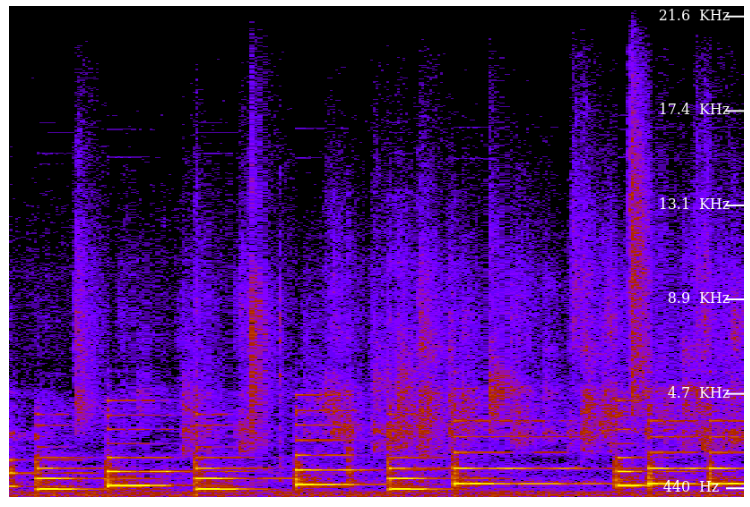
\includegraphics[width=1\columnwidth]{noisy.png}
\caption{Spectrum of noisy audio signal $\vec{x(n)}$}
\label{fig:Spectrum of noisy audio signal}
\end{figure}
\begin{flushleft}


\section{Design of 3rd order Butterworth filter}

\vspace{0.2cm}
Let the impulse response of the 3rd order butterworth filter is denoted by $\vec{h(n)}$.\\  
\vspace{0.2cm}
Let the output audio signal (filtered audio signal) is denoted by $\vec{y(n)}$.\\ 
\end{flushleft}
\vspace{0.25cm}
\subsection{Block diagram of Butterworth filter} 
\vspace{0.2cm}
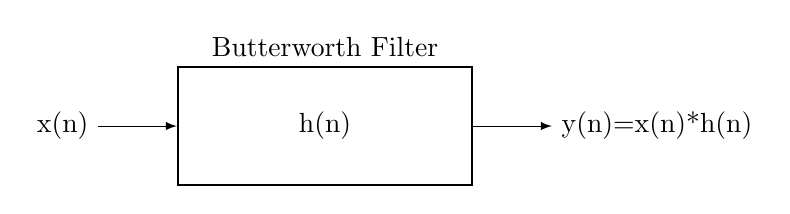
\begin{tikzpicture}  
\node[] (a) {x(n)}; 
\node[block, right=of a, label={Butterworth Filter}] (b) {h(n)};
%\node[draw,inner xsep=4mm,inner ysep=7mm,fit=(d)(e),label={80:Q}]{};  
\node[ ,right=of b] (c) {y(n)=x(n)*h(n)};
\draw[line] (a)-- (b);  
\draw[line] (b)-- (c);  
\end{tikzpicture}  
\vspace{0.2cm}
    
\begin{flushleft}
\hspace{1cm} Block diagram of Butterworth filter  \\
\end{flushleft}

\subsection{Coefficients of 3rd order Butterworth filter} 
\vspace{0.25cm}
\begin{flushleft}
General form of Difference equation for IIR filter is expressed as,\\
\begin{equation}
\sum_{k=0}^{N} {a_k} \hspace{0.1cm} {\vec{y(n-k)}}
=  \sum_{k=0}^{M} {b_k} \hspace{0.1cm} {\vec{x(n-k)}}
\end{equation}
\vspace{0.5cm} 
From equation 4.2.1, impulse response in Z-transform can be writtens as,\\
\begin{equation}
H(z)= \frac{b_0 + b_1 z^{-1} + b_2 z^{-2} + b_3 z^{-3}}{a_0 + a_1 z^{-1}+ a_2 z^{-2} + a_3 z^{-3}}
\end{equation}

For 3rd order Butterworth Digital Filter, the co-efficients can be derived from the Table of Butterworth polynomials as follows,\\
\vspace{1cm}

Denominator Coefficients:\\
\begin{center}
$a_0$= 1.00000000 \\
\vspace{0.15cm}
$a_1$=-1.87302725 \\ 
\vspace{0.15cm}
$a_2$= 1.30032695 \\
\vspace{0.15cm}
$a_3$=-0.31450204 \\
\end{center}
\vspace{0.35cm}
Numerator Coefficients:\\  
\vspace{0.1cm}
\begin{center}
    
$b_0$= 0.01409971 \\ 
\vspace{0.15cm}
$b_1$= 0.04229913 \\
\vspace{0.15cm}
$b_2$= 0.04229913 \\
\vspace{0.15cm}
$b_3$= 0.01409971 \\
\end{center}
\end{flushleft}
\begin{flushleft}
Impulse response given in equation 4.2.2 is in Z domain.\\
It can be converted into time domain by applying inverse Z-transform as,\\
\begin{flushleft}
    
$\vec{h(n)} = Z^{-1}[H(Z)]$\\
\vspace{0.2cm}
$= 0.0140997,$ for $n=0 $\\
\vspace{0.2cm}
$= (0.640832 - 3.68314*10^{(-17)}j) * 0.546882^n $\\
 $ -(0.29095 - 0.141431j) * (0.663072 - 0.36799j)^n$ \\
 $ -(0.29095 + 0.141431j) *(0.663072 + 0.36799j)^n$, for $n>0$   
\end{flushleft}

\subsection{Plot of Impulse response}
\vspace{0.2cm}
From the above equation of $\vec{h(n)}$, Impulse response is plotted using Python code. Plot of Impulse response is shown in the figure 2.\\
\begin{figure}[h]
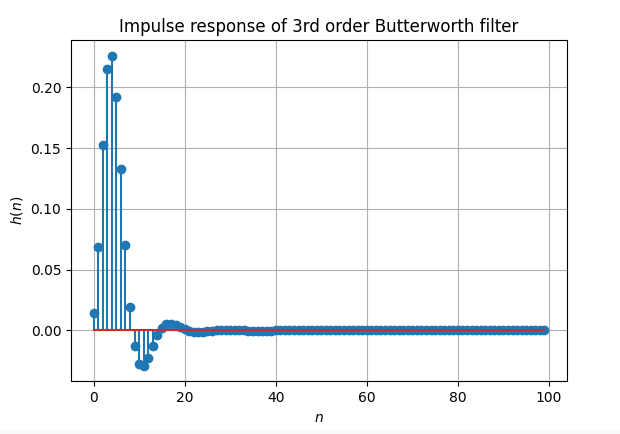
\includegraphics[width=1\columnwidth]{impulse.png}
\caption{Impulse response of 3rd order Butterworth filter}
\label{fig:Impulse response of 3rd order Butterworth filter}
\end{figure}

\subsection{Response of 3rd order Butterworth filter}
\vspace{0.2cm}
The output response can be calculated in the following Two different ways.\\
\vspace{0.2cm}
\subsubsection{Convolution process in Z-domain}
\vspace{0.2cm}
Let the given Input noisy audio signal is represented in Z-domain as $\vec{X(Z)}$ and the Impulse response as $\vec{H(Z)}$.
Then the output response of the filter can be obtained by applying Convolution process in Z-domain and taking inverse Z-transform as,\\
\begin{equation}
\vec{Y(Z)}= \vec{X(Z)} * \vec{H(Z)}
\end{equation}\\
\vspace{0.2cm}
And,
\begin{equation}
\vec{y(n)}= Z^{-1}[\vec{Y(Z)}]
\end{equation}
\vspace{0.2cm}
\subsubsection{Convolution process in Time domain}
\vspace{0.2cm}
On applying Convolution  process directly in Time domain on Input noisy audio signal $\vec{x(n)}$ and Impulse response $\vec{h(n)}$, we get,
\vspace{0.25cm}
\begin{equation}
    \vec{y(n)} = \vec{x(n)}*\vec{h(n)}
\end{equation}\\

where y(n) is the filtered signal. It is the output response of 3rd order Butterworth filter.\\
\vspace{0.3cm}
\section{Spectrum of output signal}
\vspace{0.5cm}
Audio signal derived from the equation 4.4.2 (or 4.4.3) is in time domain.\\
It is the Output response of 3rd order Butterworth filter.\\
It is a reduced noise signal.\\
\vspace{0.2cm}
After applying this output signal on Spectrum analyzer, we will get the Spectrum of the output response of 3rd order Butterworth filter and it is shown in figure 3.\\
\vspace{0.2cm}
From the figure 3, it can be noticed that the noise is reduced upto 4kHz.\\
\end{flushleft}

\begin{figure}[h]

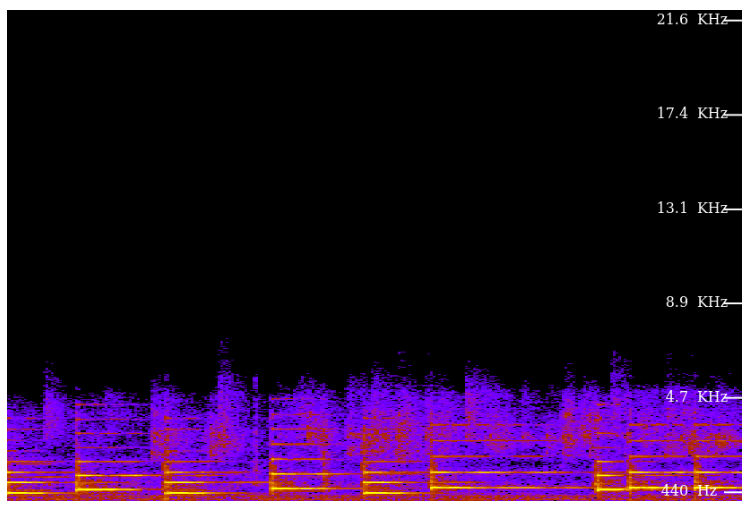
\includegraphics[width=1\columnwidth]{filtered.png}
\caption{Spectrum of output audio signal $\vec{y(n)}$}
\label{fig:Spectrum of output audio signal}
\end{figure}

\section{Code in Python language}
\centering
Python code can be downloaded from the following link.
\begin{table}[h]
\centering
\begin{tabular}{|c|} \hline
\rule{0pt}{10pt} 
https://github.com/meertabresali-FWC-IITH/\\
/Module2/blob/master/ButterworthFilter/codes/\\
ButterworthFilter.py\\
\\\hline
 \end{tabular}
\end{table}

\section{Conclusion}
\begin{flushleft}

This research work, can be concluded with the following points.\\
\vspace{0.1cm}

%1. In any communication system, during the transmission of the signal, or while receiving the signal, noise signal gets introduced into the communication.

1. Noise is an unwanted signal which interferes and corrupts the parameters of the message signal. This alteration in the message signal, leads to the disturbance and degrades the quality of the signal. \\
\vspace{0.2cm}
2. In general, for removal of the noise, various filters are used. But, still there are chances of noise in the filtered signal. \\ 
\vspace{0.2cm}
3. In the present research work, a noisy audio signal (tone) in wav format is taken as message signal.\\
\vspace{0.2cm}
4. It has been aimed to remove the noise upto 3rd order as this can reduce the noise as maximum as possible. \\
\vspace{0.2cm}
5. For achieving this, Butterworth filter has been designed by defining its impulse response upto 3rd order and then the noise is removed by using Convolution process. \\
\vspace{0.2cm}
6. The codes have been written in Python language and the output signal is generated by running the Python codes. \\
\vspace{0.2cm}
7. Input and output signals are taken on spectrum analyser. The spectrum of output signal can bee seen noise free. 
\end{flushleft}

\section{References}
\begin{flushleft}
    

\vspace{0.2cm}
1. Introduction to Digital filters with Audio applications: JULIUS O. SMITH, Center for Computer Research in Music and Acoustics (CCRMA), https://ccrma.stanford.edu/~jos/filters/ \\
\vspace{0.25cm}
2. Design of IIR filters: University of Newcastle upon Tyne, Chapter 5, $https://www.staff.ncl.ac.uk/oliver.hinton/eee305/Chapter5.pdf$\\
\vspace{0.25cm}
3. Digital Signal Processing : by Proakis and Manolokis\\
\vspace{0.25cm}
4. Introduction to Signal Processing: by Sophocles J. Orfanidis, Rutgers University, http://www.ece.rutgers.edu/~orfanidi/intro2spRutgers University\\
\vspace{0.25cm}
5. Digital Signal Processing: IIR Filters design, $https://getmyuni.azureedge.net/assets/main/study-material/notes/computer-science_engineering_digital-signal-processing_iir-filter-design_notes.pdf$\\
\vspace{0.20cm}
6. IIR filters structures: Miodrag Bolic,  $http://web.cecs.pdx.edu/~mperkows/CAPSTONES/DSP1/$ \\
$ELG6163_IIR.pdf$\\
\vspace{0.25cm}
7. Digital Signal Processing : by S K Mitra\\
\vspace{0.25cm}
8. Digital Signal Processing : by A Nagoor Kani\\
\vspace{0.25cm}
9. Digital Signal Processing : by A Anand Kumar\\
\vspace{0.25cm}
10. Schaum's Outline of Theory and Problems of Digital Signal Processing : by Monson H Hayes\\
\vspace{0.25cm}
11. $https://en.wikipedia.org/wiki/Butterworth_filter$\\
\vspace{0.25cm}
12. $https://www.electronics-tutorials.ws/filter/filter_8.html$\\
\vspace{0.25cm}
13. Butterworth-Filter-Design:ruohoruotsi, $https://github.com/ruohoruotsi/Butterworth-Filter-Design$\\
\vspace{0.25cm}
14. Butterworth-filter: arasgungore, $https://github.com/arasgungore/butterworth-filter$\\
\vspace{0.25cm}
15. $https://www.geeksforgeeks.org/digital-low-pass-butterworth-filter-in-python/$\\
\vspace{0.25cm}
\end{flushleft}
\begin{center}
*-*-*-*-*
\end{center}
\end{document}
